

%======================================================================
\newpage
\section{Tesztelés}
\label{sec:testing}
%======================================================================

\subsection{Tesztelési terv}
\label{sec:testplan}

A fejlesztés során kiemelt szempont volt, hogy a rendszer ne csak jól használható felületet biztosítson,
 hanem a mögötte működő algoritmusok is helyes eredményeket adjanak.
Mivel az alkalmazás oktatási célokat szolgál, egy kisebb hiba nem csupán működési problémát jelenthet, hanem hibás vagy félrevezető tananyag megjelenéséhez is vezethet. Ennek megfelelően a tesztelés elsődleges célja az algoritmusok helyességének igazolása, valamint a funkcionális és nem funkcionális követelmények teljesülésének ellenőrzése.


A projekt pnpm monorepo struktúrában valósul meg, ahol az algoritmusokat megvalósító automata-core 
csomag elkülönül a React alapú felhasználói felülettől. A rendszer kliensoldalon fut,
a tesztelés az algoritmusokra, a modulok együttműködésére és a felhasználói folyamatok helyességére összpontosít.


A tesztelési stratégia több szintből áll.
Az egységtesztek az egyes algoritmusok helyességét, az integrációs tesztek a modulok együttműködését,
míg a végponttól végpontig (E2E) tesztek a teljes felhasználói folyamatok működését vizsgálják.
A stratégia a tesztelési piramis elvét követi, ezért a tesztek többségét egységtesztek alkotják, 
amelyeket kisebb számú integrációs és E2E teszt egészít ki.





\begin{figure}[H]
    \centering
    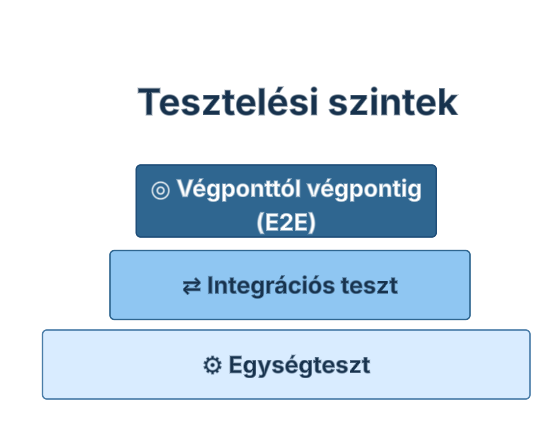
\includegraphics[width=0.5\textwidth]{tesztelesi_szintek.png}
    \caption{Tesztelési szintek}
    \label{fig:tesztelesi_szintek}
\end{figure}

\newpage
\subsubsection{Automatizált futtatás}

A tesztek fejlesztése Windows 11 környezetben történt,
Ubuntu Linux virtuális környezetben GitHub Actions alatt automatikus futtnak minden a master branchre tórténő commitot követően.

 A projekt Node.js~24 futtatókörnyezetet használ. 
 Külső adatbázis vagy egyéb szolgáltatás nem szükséges, 
 mivel a rendszer minden számítást memóriában végez.
  
TODO
 mostani unit + integration + E2E rendszer,
-2 property based teszt fast-check-kel,
emeld ki a cross-validation és regressziós teszteket a szövegben.
UI tesztek?


\subsubsection{Elfogadási feltétel}

A tesztelés akkor tekinthető sikeresnek, ha minden automatizált teszt
hibátlanul lefut, minden E2E teszteset az elvárt eredményt adja
három támogatott böngészőben, és nincs olyan ismert hiba, amely hibás
eredményt mutatna a hallgatónak. 

\subsection{ Unit testing - Egységtesztek}

Az egységtesztek  az \texttt{automata-core} csomag minden
függvényét elszigetelten, az összes többi modultól függetlenül
ellenőrizik. A tesztek a Node.js beépített \texttt{node:test}
keretrendszerével valósultak meg.
Külső könyvtár nélkül az elvárt értékek
összehasonlítására a \texttt{node:assert/strict} modult szolgált.
 Az összes automatikus teszt a következő paranccsal futtatható: 
 \begin{verbatim} 
    pnpm --filter @fotoc/automata-core test 
\end{verbatim}

\subsubsection*{Lefedettség}
A 12 darab unit teszt a \path{packages/automata-core/test/} mappában találhatók
és a csomag összes nyilvánosan exportált
függvényét lefedik. A tesztesetek kiválasztásakor a szemantikailag
érdekes esetekre, köztük az előadáson bemutatott néhány
példákra, valamint a hibás bemenetekre és a határesetekre fordult hangsúly.
(\ref{fig:test-structure}.~ábra).

\begin{figure}[htbp]
\centering
\begin{minipage}{0.85\textwidth}
\dirtree{%
.1 packages/.
.2 automata-core/.
.3 test/.
.4 chomsky.test.ts\DTcomment{Chomsky normálforma}.
.4 cyk.test.ts\DTcomment{CYK algoritmus}.
.4 dfa.test.ts\DTcomment{Determinisztikus véges automata}.
.4 grammer.test.ts\DTcomment{Nyelvtanok}.
.4 language.test.ts\DTcomment{Nyelvek műveletei}.
.4 logic.test.ts\DTcomment{Logikai segédfüggvények}.
.4 minimize.test.ts\DTcomment{DFA minimalizálás}.
.4 nfa.test.ts\DTcomment{Nemdeterminisztikus véges automata}.
.4 normalform3.test.ts\DTcomment{3-as normálformára hozás}.
.4 turing.test.ts\DTcomment{Turing-gép}.
.4 verem.test.ts\DTcomment{Veremautomata}.
.4 words.test.ts\DTcomment{Szavak műveletei}.
}
\end{minipage}
\caption{Az \texttt{automata-core} csomag tesztfájljai}
\label{fig:test-structure}
\end{figure}



A tesztek a csomag moduljait négy tematikus csoport szerint mutatják be.

\begin{figure}[H]
\centering
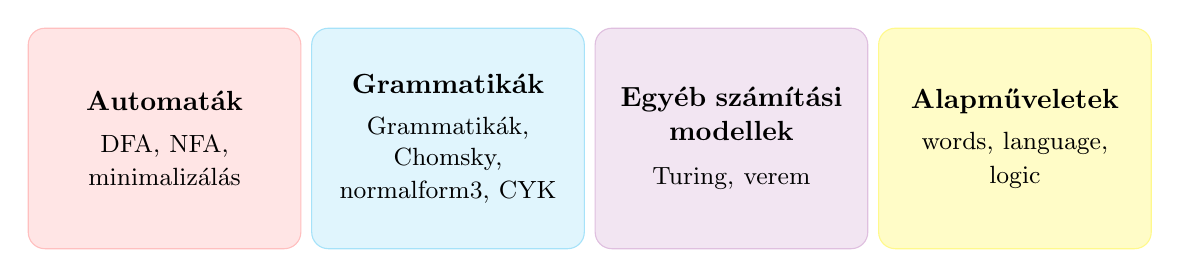
\begin{tikzpicture}[
  grp/.style={
    rectangle, rounded corners=6pt,
    minimum width=3.1cm, minimum height=2.8cm,
    text width=2.9cm, align=center, inner sep=8pt
  }
]
  \node[grp, fill=red!10, draw=red!25] at (0,0)
    {\textbf{Automaták}\\[4pt]{\small DFA, NFA,\\minimalizálás}};
  \node[grp, fill=cyan!12, draw=cyan!35] at (3.6,0)
    {\textbf{Grammatikák}\\[4pt]{\small Grammatikák,\\Chomsky,\\normalform3, CYK}};
  \node[grp, fill=violet!10, draw=violet!25] at (7.2,0)
    {\textbf{Egyéb számítási modellek}\\[4pt]{\small Turing, verem}};
  \node[grp, fill=yellow!22, draw=yellow!45] at (10.8,0)
    {\textbf{Alapműveletek}\\[4pt]{\small words, language,\\logic}};
\end{tikzpicture}
\caption{Az egységtesztek tematikus csoportjai}
\label{fig:test-groups}
\end{figure}

\newpage

\paragraph{Automaták}
Az automaták csoport tesztjei a DVA, NDVA és DFA-minimalizáló modulok 
legfontosabb funkcióit fedik le. A tesztek ellenőrzik az automaták szimulációit, 
az elfogadási eredmények helyességét, az ε-átmenetek kezelését, a különböző
automatatípusok közötti átalakításokat, valamint a minimalizálási algoritmus 
működését.
Kiemelt szempont, hogy az átalakítások ne változtassák meg a felismert nyelvet.
\begin{table}[H]
    \centering
    \begin{tabularx}{\textwidth}{|l|l|X|}
        \hline
        \textbf{Modul} & \textbf{Tesztcsoport} & \textbf{Leírás} \\ \hline
        \texttt{dfa.ts} & isComplete & Az automata teljességének ellenőrzése. Minden állapotból létezzen átmenet minden szimbólumra \\ \hline
        \texttt{dfa.ts} & runDfa & DFA futás szimulációja, az elfogadás helyessége, a futási nyomvonal konzisztenciája \\ \hline
        \texttt{dfa.ts} & Hibakezelés & Ábécén kívüli szimbólumok felismerése. \\ \hline
        \texttt{dfa.ts} & dfaToNfa & DVA-->NFA átalakítás szerkezeti és átmeneti helyessége. \\ \hline
        \texttt{nfa.ts} & epsilonClosure & Az ε-lezárt kiszámítása ε-mentes, láncos és köröses esetben. \\ \hline
        \texttt{nfa.ts} & runNfa & állapothalmazok lépésenkénti változásának ellenőrzése. \\ \hline
        \texttt{nfa.ts} & acceptsWord & Elfogadási feltétel vizsgálata normál, üres szavas és ε-átmenetes esetekben. \\ \hline
        \texttt{nfa.ts} & determinize & Részhalmaz-konstrukció, csapdaállapot, sorbanállás kezelése. \\ \hline
        \texttt{minimize.ts} & reachableLayers & Elérhetetlen állapotok rétegenkénti eltávolítása. \\ \hline
        \texttt{minimize.ts} & equivalenceRounds & Ekvivalenciaosztályok iteratív finomítása. \\ \hline
        \texttt{minimize.ts} & minimize & Állapotszám, eltávolított állapotok, nyelvazonosság. \\ \hline
    \end{tabularx}
    \caption{Az automaták csoportjának egységtesztjei}
    \label{tab:test_automata}
\end{table}

\newpage
\paragraph{Kiemelt teszteset} A \texttt{minimize} egyik tesztje A teszt az eredeti és a minimalizált DFA-t ugyanazon bemeneteken futtatja, és ellenőrzi, hogy minden esetben azonos elfogadási eredményt adnak. Ez igazolja, hogy a minimalizálás nem változtatja meg a felismert nyelvet.
\begin{lstlisting}
    const lectureExample: Dfa = {
  states: ["q0", "q1", "q2", "q3", "q4", "q5", "q6"],
  alphabet: ["a", "b"],
  start: "q0",
  accepting: ["q2", "q5"],
  transitions: {
    q0: { a: "q1", b: "q3" },
    q1: { a: "q4", b: "q2" },
    q2: { a: "q4", b: "q3" },
    q3: { a: "q4", b: "q0" },
    q4: { a: "q1", b: "q5" },
    q5: { a: "q1", b: "q0" },
    q6: { a: "q2", b: "q6" },
  },
};
describe("minimize", () => {
  const { minimal, removed } = minimize(lectureExample);
  ...

  test("ugyanazt a nyelvet ismeri fel", () => {
    for (const word of ["", "a", "b", "ab", "aab", "abb", "bab", "abab", "ba"]) {
      assert.equal(runDfa(minimal, word).accepted, runDfa(lectureExample, word).accepted, word);
    }
  });
  ...
});
\end{lstlisting}

\newpage

\paragraph{Grammatikák}
A grammatikák csoport egységtesztjei a levezetési algoritmusok,
 a Chomsky-féle nyelvosztályozás, a 3-as normálformára alakítás 
 és a CYK-felismerő algoritmus helyességét vizsgálják. 
 A tesztek ellenőrzik a szabályalkalmazások működését, 
 a nyelvtanok osztályozását, az átalakítások nyelvmegőrző tulajdonságát,
  valamint a szavak felismerésének és levezetésének helyességét a különböző esetekben.
\begin{table}[H]
    \centering
    \begin{tabularx}{\textwidth}{|l|l|X|}
        \hline
        \textbf{Modul} & \textbf{Tesztcsoport} & \textbf{Leírás} \\ \hline
        \texttt{grammer.ts} & possibleSteps & Lehetséges szabályalkalmazások meghatározása, több előfordulású nemterminálisok kezelése. \\ \hline
        \texttt{grammer.ts} & applyStep & Szabályalkalmazás helyessége a szó elején, közepén és végén. \\ \hline
        \texttt{grammer.ts} & isTerminalWord & Terminális és nemterminális mondatformák felismerése. \\ \hline
        \texttt{chomsky.ts} & classifyGrammer & Teljes nyelvtanok Chomsky-besorolása. \\ \hline
        \texttt{chomsky.ts} & checkOneRule & Egyedi szabályok típusbesorolása Chomsky-hierarchiában. \\ \hline
        \texttt{chomsky.ts} & Példanyelvtanok & Előadásból és ZH-ból vett grammatikák besorolásának validálása. \\ \hline
        \texttt{chomsky.ts} & tokenize / Hibakezelés & Tokenizálás és hibás szabályok kezelése. \\ \hline
        \texttt{normalform3.ts} & lengthReduction & Hosszú jobboldalú szabályok rövidítése, nyelv megőrzése. \\ \hline
        \texttt{normalform3.ts} & chainLayers / removeChains & Láncszabályok lezártja és eltávolítása. \\ \hline
        \texttt{normalform3.ts} & Nyelvmegőrzés & Az átalakítás ekvivalenciájának ellenőrzése. \\ \hline
        \texttt{normalform3.ts} & toNormalForm3Steps & Teljes átalakítási folyamat lépéseinek validálása. \\ \hline
        \texttt{cyk.ts} & isChomskyNormalForm & CNF-feltételek ellenőrzése (ε, lánc, jobboldal hossza). \\ \hline
        \texttt{cyk.ts} & cyk & Elfogadás/elutasítás, üres szó, táblázatméret. \\ \hline
        \texttt{cyk.ts} & cykDerivation & Visszakövetett levezetési sorozat érvényessége. \\ \hline
    \end{tabularx}
    \caption{A grammatikák csoportjának egységtesztjei}
    \label{tab:test_grammar_group}
\end{table}

\newpage
\paragraph{Kiemelt teszteset} A \texttt{normalform3.ts} modul \texttt{chainLayers} függvényének következó tesztje egy körkörös láncszabálysorozatot ($S \to A \to B \to S$) tartalmazó grammatikán ellenőrzi, hogy a lezárt kiszámítása mégis megáll, és minden ciklusbeli nemterminális bekerül a halmazba. Ez azért fontos, mert hibás megvalósítás esetén végtelen bejáráshoz vagy hiányos eredményhez vezethet.
\begin{lstlisting}
test("láncciklus: megáll, és mindenki benne van", () => {
  const g = grammar(["S->A", "A->B", "B->S", "B->a"], ["S", "A", "B"]);
  assert.deepEqual(sortedLayers(chainLayers(g, "S")),
    [["S"], ["A", "S"], ["A", "B", "S"]]);
  assert.deepEqual(sortedLayers(chainLayers(g, "B")),
    [["B"], ["B", "S"], ["A", "B", "S"]]);
});
\end{lstlisting}

\paragraph{Egyéb számítási modellek}
A csoport a Turing-gép és a veremautomata szimulátorok tesztjeit foglalja össze. A tesztek a konfigurációk és átmenetek kezelését, a futások szimulációját, valamint az elfogadási feltételek ellenőrzését vizsgálják.

\begin{table}[H]
    \centering
    \begin{tabularx}{\textwidth}{|l|l|X|}
        \hline
        \textbf{Modul} & \textbf{Tesztcsoport} & \textbf{Leírás} \\ \hline
        \texttt{turing.ts} & initConfiguration & Kezdőkonfiguráció előállítása üres és nemüres bemeneten. \\ \hline
        \texttt{turing.ts} & isHalted / isAccepted & Megállási és elfogadási feltételek ellenőrizése. \\ \hline
        \texttt{turing.ts} & findTransition & Illeszkedő és hiányzó átmenetek kezelése. \\ \hline
        \texttt{turing.ts} & step & Egy lépés végrehajtása, a szalag kétirányú bővítésének kezelése. \\ \hline
        \texttt{turing.ts} & computeAllSteps & Teljes futássorozat és lépésszámkorlát kezelése. \\ \hline
        \texttt{verem.ts} & parsePdaRules & Veremautomata szabályok feldolgozása ésnhibás sorok felismerése \\ \hline
        \texttt{verem.ts} & konfigurációk & Kezdőkonfiguráció, konfigurációmódosítás és egyedi azonosítás ellenőrzése.\\ \hline
        \texttt{verem.ts} & epsilonClosure & ε-lépések lezártja, körnél megállás, végtelen növekedés levágása. \\ \hline
        \texttt{verem.ts} & wordchecker & Elfogadás és elutasítás vizsgálata különböző elfogadási módok esetén. \\ \hline
        \texttt{verem.ts} & runningPda és utak & Elfogadó és legjobb futási utak meghatározása. \\ \hline
        \texttt{verem.ts} & isDeterministic & A determinisztikusság feltételének ellenőrzése. \\ \hline
        \texttt{verem.ts} & findPdaCounterexample & Ellenpélda-keresés és eldönthetetlen esetek számlálása. \\ \hline
    \end{tabularx}
    \caption{Az egyéb modellek csoportjának egységtesztjei}
    \label{tab:test_models}
\end{table}

\paragraph{Kiemelt teszteset} A \texttt{verem.ts} modul egyik tesztje egy olyan PDA-t vizsgál, amelynek egyetlen szabálya ($\# \, q \to \# \, \# \, q$) ε-lépésenként növeli a vermet. A teszt ellenőrzi, hogy az \texttt{epsilonClosure} a \texttt{maxStack} korlát elérésekor leáll, és a \texttt{truncated} jelzőt igazra állítja.
\begin{lstlisting}
const pumpForever = pdaFrom(`# q -> # # q`, "#", "q", ["f"]);

test("végtelen veremnövelésnél levág és jelzi", () => {
  const { configs, truncated } =
    epsilonClosure(pumpForever, [startConfig(pumpForever)], LIMITS);
  assert.equal(truncated, true);
  assert.ok(configs.every((c) => c.stack.length <= LIMITS.maxStack));
});
\end{lstlisting}

\paragraph{Alapműveletek}
Az utolsó csoport három, egymástól független területet fed le: a szóoperációkat (\texttt{words.ts}), a reguláris kifejezések elemzését és illesztését (\texttt{language.ts}), valamint a propozicionális logika kiértékelését (\texttt{logic.ts}).

\begin{table}[H]
    \centering
    \begin{tabularx}{\textwidth}{|l|l|X|}
        \hline
        \textbf{Modul} & \textbf{Tesztcsoport} & \textbf{Leírás} \\ \hline
        \texttt{words.ts} & reverse / concatenate / power & Szó megfordítása, összefűzés, hatványozás helyessége. \\ \hline
        \texttt{words.ts} & prefixes / suffixes & Prefix- és szuffixhalmazok előállítása. \\ \hline
        \texttt{words.ts} & runAll & Az összes szóoperáció együttes ellenőrzése. \\ \hline
        \texttt{language.ts} & shortlex & Shortlex sorrend szerinti szógenerálás. \\ \hline
        \texttt{language.ts} & Parser & Reguláris kifejezések elemzése és hibakezelés. \\ \hline
        \texttt{language.ts} & regexMatches / findRegexCounterexample & Illeszkedés és ekvivalencia-ellenőrzés. \\ \hline
        \texttt{language.ts} & checkRegex & Hallgatói megoldások automatikus ellenőrzése. \\ \hline
        \texttt{language.ts} & NFA-konverzió & Reguláris kifejezés → NFA konzisztencia. \\ \hline
        \texttt{logic.ts} & parseFormula & Formulaelemzés, precedencia, Unicode-jelkezelés. \\ \hline
        \texttt{logic.ts} & truthTable & Igazságtáblázat, osztályozás, KNF-generálás. \\ \hline
    \end{tabularx}
    \caption{Az alapműveletek csoportjának egységtesztjei}
    \label{tab:test_basic}
\end{table}

\paragraph{Kiemelt teszteset} A \texttt{logic.ts} modul tesztje az előadás feladatának ($y \to x \land \lnot y \lor \lnot z$) teljes igazságtáblázatát ellenőrzi: a változók sorrendjét, a közbülső oszlopok neveit, és az utolsó oszlop összes sorigazságértékét. Ezzel nem csupán a végeredmény, hanem a közbülső kiértékelési lépések helyessége is igazolt.
\begin{lstlisting}
test("minta 1. feladat", () => {
  const table = truthTable(parse("y -> x & ~y | ~z"));
  assert.deepEqual(table.variables, ["y", "x", "z"]);
  assert.deepEqual(table.columns.map(formulaToString),
    ["¬y", "¬z", "x ∧ ¬y", "x ∧ ¬y ∨ ¬z", "y → x ∧ ¬y ∨ ¬z"]);
  const last = table.rows.map((row) => (row.values[4] ? "i" : "h")).join("");
  assert.equal(last, "hihiiiii");
});
\end{lstlisting}

\subsection{Integrációs tesztek}
A unit tesztek már bizonyították az egyes algoritmusok függvényei önállóan jól működnek, pont ahogy mi elvárjuk.
Nézzük meg integrációs szinten, hogy az egymásra épülő komponensek
 helyesen működnek-e együtt. 
 Az Integrációs tesztelés a különálló modulok összekapcsolása után azok 
 együttműködésének ellenőrzését jelenti. 
 A jelen rendszerben ez elsősorban az elemzők, algoritmusok és 
 transzformációs lépések közötti adatátadás, 
 valamint a több lépésből álló feldolgozási láncok konzisztenciájának
  vizsgálatát jelenti.
Az integrációs tesztek az \texttt{integration.test.ts} fájlban találhatók,
 és két kategóriába sorolhatók: 
 az első kategória az elemzők és az algoritmusok együttműködését vizsgálja,
  a második a több transzformációs lépésből álló pipeline-ok ekvivalenciáját 
  ellenőrzi. 
  Mindkét kategória a \texttt{// \#INT} jelöléssel ellátott 
  teszteseteket is tartalmazza, 
  amelyek az egységtesztek között korábban azonosított integrációs 
  pontokat egészítik ki.

\subsubsection*{Elemző és algoritmus}
Az első csoport olyan tesztekből áll, 
ahol egyik komponens kimenete egy másik komponens bemenetévé válik.
A cél annak ellenőrzése és verifikálása, hogy a komponensek közötti 
adatátadás és reprezentáció nem sérül a feldolgozás során.

Itt azok a tesztek vannak, amelyek szöveges bemenetet értelmeznek, majd az ebből előállított
 adatszerkezetet egy algoritmusnak adják át.

\begin{table}[H] \centering \begin{tabularx}{\textwidth}{|l|X|} \hline \textbf{Tesztcsoport} & \textbf{Leírás} \\ \hline \texttt{[INT] parsePdaRules → wordchecker} & Szöveges PDA-leírás feldolgozása után az elfogadási és elutasítási eredmények ellenőrzése $a^nb^n$ és $wcw^R$ nyelveken. \\ \hline \texttt{[INT] parseRegex → regexToNfa → nfaAccepts} & Szöveges reguláris kifejezés elemzése, NFA-vá alakítása és az NFA elfogadási viselkedésének ellenőrzése. \\ \hline \end{tabularx} \caption{Elemző–algoritmus integrációs tesztek} \label{tab:int_parser} \end{table}
\paragraph{Kiemelt teszteset} A \texttt{regexToNfa} integrációs teszt az összes legfeljebb 6 betű hosszú szóra ellenőrzi, hogy a reguláris kifejezés közvetlen kiértékelése (\texttt{regexMatches}) és a reguláris kifejezésből előállított NFA szimulációja (\texttt{nfaAccepts}) ugyanazt az eredményt adja-e. A teszt ezzel egyszerre validálja a parser, az automataépítő algoritmus és az automata szimuláció együttműködését.

\begin{figure}[H]
    \centering
    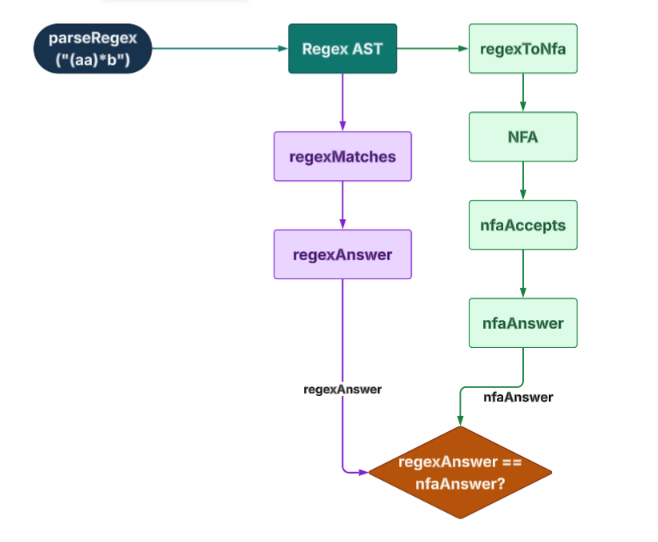
\includegraphics[width=0.7\textwidth]{images/image2.png}
    \caption{A parseRegex, regexToNfa és nfaAccepts komponensek integrációjának ellenőrzése}
    \label{fig:tesztelesi_szintek}
\end{figure}

\newpage
\begin{lstlisting} 
    test("regexToNfa konzisztens a regexMatches-szel n hosszig", function () {
        const result = parseRegex("(aa)*b");
        if (!result.ok) {
        throw new Error("'(aa)*b' nem értelmezhető");
        }
        const regex = result.regex;
        const nfa = regexToNfa(regex);
        const allWords = shortlex(["a", "b"], 6);

        for (const word of allWords) {
        const nfaAnswer = nfaAccepts(nfa, word);
        const regexAnswer = regexMatches(regex, word);
        assert.equal(nfaAnswer, regexAnswer, word);
        }
    });
\end{lstlisting}

\subsubsection*{Több transzformációs lépés egymás után}

A második csoportban több egymást követő transzformáció alkot feldolgozási láncot. Ezeknél nem az egyes lépések helyessége a fő kérdés, hanem az, hogy a teljes átalakítási folyamat megőrzi-e a leírt nyelvet.
alakítanak. Az Vagyis akkor helyes, ha a kapott objektum ugyanazt a nyelvet írja le, mint a kiindulási.

\begin{table}[H] \centering \begin{tabularx}{\textwidth}{X X} \hline 
    \textbf{Tesztcsoport} & \textbf{Leírás} \\ \hline 
    \texttt{[INT] DFA → dfaToNfa → determinize} & A körmenet (DFA→NFA→DFA) után az elfogadási viselkedés 
    megőrzésének ellenőrzése. \\ \hline 
    \texttt{[INT] Grammar → classifyGrammer → isChomskyNormalForm → cyk} & 
    Háromfázisú pipeline: besorolás, CNF-ellenőrzés, CYK-futtatás konzisztenciájának vizsgálata. \\ \hline 
    \texttt{[INT] cyk → cykDerivation} & A visszakövetett levezetési sorozat minden lépésének érvényes 
    szabályalkalmazásra ellenőrzése. \\ \hline 
    \texttt{[INT] Grammar → toNormalForm3Steps} & A 3-as normálformára hozás után a generált szavak 
    halmazának összehasonlítása az eredeti grammatikáéval. \\ \hline 
\end{tabularx} 
\caption{Transzformációs pipeline integrációs tesztek} 
\label{tab:int_pipeline} 
\end{table}

\paragraph{Kiemelt teszteset} A \texttt{cyk} és \texttt{cykDerivation} modulokat összekötő teszt ellenőrzi, 
hogy a visszakövetett levezetési sorozat $S$-sel kezd, 
a célszóval végez, és közbülső lépésenként egy érvényes szabályalkalmazásnak felel meg.
 Az \texttt{isValidStep} segédfüggvény a grammatika szabályait iterálja, és csak azt a lépést fogadja el,
  amelynél valamelyik szabály pontosan a megfigyelt csere. 
Ez a teszt azért fontos, mert a \texttt{cykDerivation} közvetlenül a \texttt{cyk} által előállított táblázatra
 épül, és az egységtesztek önmagukban nem garantálják, hogy a két komponens között 
 átadott adatszerkezet minden esetben kompatibilis marad.
\begin{figure}[H] 
    \centering 
    \makebox[\textwidth][c]{% 
    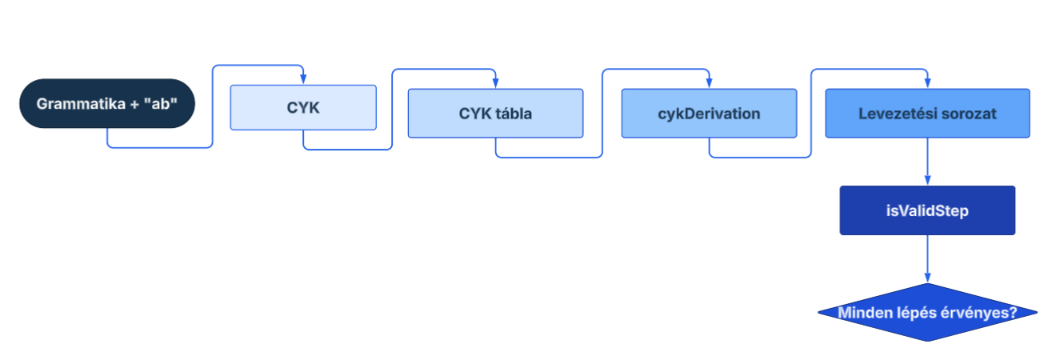
\includegraphics[width=1.3\textwidth]{images/image.png} } 
    \caption{A CYK és a levezetés-visszakövető modul közötti integráció.} 
    \label{fig:cyk_derivation} 
\end{figure}

\begin{lstlisting}
  for (const word of ["a", "ab"]) {
    test(`"${word}": a levezetés S-sel kezd, a szóval végez, minden lépés érvényes`, () => {
      const r = cyk(g, word);
      assert.ok(r.ok);
      if (!r.ok) return;

      const d = cykDerivation(g, word, r.table);
      assert.ok(d !== null && d.length >= 2);
      assert.equal(d![0], g.start);
      assert.equal(d![d!.length - 1], word);
      for (let i = 0; i < d!.length - 1; i++) {
        assert.ok(isValidStep(d![i], d![i + 1]), `${d![i]} → ${d![i + 1]} nem érvényes lépés`);
      }
    });
  }
\end{lstlisting}

\subsection{E2E tesztek user interface}
\iffalse
\label{sec:e2e}
Az E2E teszteseteket a telepített alkalmazáson, Chrome, Edge és
Firefox böngészőben hajtom végre. Egy teszteset akkor sikeres, ha a
tényleges eredmény megegyezik az elvárttal, és a böngésző konzolján nem
jelenik meg hiba.

% Eredmény oszlop: kitöltendő a tesztek lefuttatása után.
\begin{table}[H]
    \centering
    \small
    \begin{tabularx}{\textwidth}{|l|X|X|c|}
        \hline
        \textbf{Azonosító} & \textbf{Lépések} & \textbf{Elvárt eredmény} &
        \textbf{Eredmény} \\ \hline
        E2E-1 (FK-4, FK-5) &
        DVA megadása, egy szó beírása, lejátszás előre és vissza
        lépésenként. &
        Minden lépésben az aktuális állapot ki van emelve, a végén
        megjelenik, hogy a szót elfogadja-e. & \\ \hline
        E2E-2 (FK-4, FK-5) &
        NDVA megadása $\varepsilon$-átmenettel, egy szó lépésenkénti
        lejátszása. &
        Minden lépésben az aktuális állapothalmaz ($\varepsilon$-lezárttal)
        látszik, az eredmény helyes. & \\ \hline
        E2E-3 (FK-6, NFK-2) &
        Hibás reguláris kifejezés (pl.\ nyitott zárójel) megadása. &
        Érthető hibaüzenet jelenik meg, az oldal működőképes marad. & \\ \hline
        E2E-4 (FK-5) &
        Két reguláris kifejezés ekvivalenciájának vizsgálata, egyszer
        ekvivalens, egyszer nem ekvivalens párral. &
        Ekvivalens párnál ezt jelzi, különben egy ellenpélda szót mutat. & \\ \hline
        E2E-5 (FK-5) &
        Grammatika megadása és osztályozása a Chomsky-hierarchiában. &
        A legszűkebb osztály és az indoklás jelenik meg. & \\ \hline
        E2E-6 (FK-4, FK-5) &
        Grammatika 3-as normálformára hozása lépésenként. &
        A hosszredukció és a láncszabályok elhagyása külön lépésként
        látszik, a végeredmény 3-as normálformájú. & \\ \hline
        E2E-7 (FK-4, FK-5) &
        Chomsky-normálformájú grammatika és egy szó megadása a CYK
        modulban. &
        A táblázat lépésenként kitöltődik, az eredmény helyes. & \\ \hline
        E2E-8 (FK-4, FK-5) &
        Veremautomata szabályainak és egy szónak a megadása, futtatás. &
        A konfigurációk sorozata látszik, az elfogadás helyes. & \\ \hline
        E2E-9 (FK-4, FK-5) &
        DVA minimalizálása. &
        Az ekvivalens állapotok összevonása lépésenként látszik, az
        eredmény minimális. & \\ \hline
        E2E-10 (FK-6) &
        Hibás grammatikaszabály (pl.\ hiányzó nyíl) megadása. &
        Hibaüzenet jelenik meg, az oldal működőképes marad. & \\ \hline
        E2E-11 (FK-7) &
        Egy témakör kvízének kitöltése jó és rossz válaszokkal. &
        Minden kérdésnél visszajelzés a helyes válasszal. & \\ \hline
        E2E-12 (FK-1, FK-2, FK-8) &
        Témakör megnyitása, majd az oldal újratöltése. &
        Az elmélet és a modul megjelenik, a témakör meglátogatottként
        megmarad. & \\ \hline
    \end{tabularx}
    \caption{E2E tesztesetek}
    \label{tab:e2e}
\end{table}
\fi
\subsection{Nem funkcionális tesztek}
% Válaszidő (NFK-1), böngészők (NFK-3), reszponzivitás.
\mbox{}
\subsubsection{A követelmények és a tesztek kapcsolata - 8. Requirements Traceability}

\begin{table}[H]
    \centering
    \begin{tabularx}{\textwidth}{|l|X|}
        \hline
        \textbf{Követelmény} & \textbf{Ellenőrzés módja} \\ \hline
        FK-1, FK-2, FK-3 & integrációs teszt (tananyag), E2E teszt \\ \hline
        FK-4 & egységteszt (lépéslisták), E2E teszt
        (előre- és visszalépés) \\ \hline
        FK-5 & egységteszt, integrációs teszt (bemenetek feldolgozása,
        kereszt-ellenőrzés) \\ \hline
        FK-6, NFK-2 & egységteszt (hibás bemenetek), E2E teszt \\ \hline
        FK-7 & integrációs teszt (kvízkérdések), E2E teszt \\ \hline
        FK-8 & E2E teszt (újratöltés után) \\ \hline
        NFK-1, NFK-3 & nem funkcionális teszt \\ \hline
        NFK-4 & a tesztpéldák az előadás jelölését követik \\ \hline
        NFK-5 & a tesztek böngésző nélkül futtathatók \\ \hline
    \end{tabularx}
    \caption{Követelmények és tesztelési szintek}
    \label{tab:testtrace}
\end{table}

\subsection{Bugs Found and Fixes}

\subsection{A tesztelés értékelése}
\label{sec:testeval}
% Lefedettség, ismert hibák, korlátok.
\mbox{}
